\label{ap:galeria_interfaces}
Este apéndice recopila las capturas de pantalla de la interfaz de usuario (UI) y los entornos visuales del prototipo de \textit{Reset}. Las imágenes ilustran la dirección de arte en pixel art y las diferentes pantallas que componen la experiencia de usuario (UX).

% =========================================================================
\section{Menú Principal de Reset}
Esta sección muestra las pantallas del menú principal del juego, las cuales simulan la estética y gráficos de una pantalla clásica:

\begin{figure}[htbp]
    \centering
    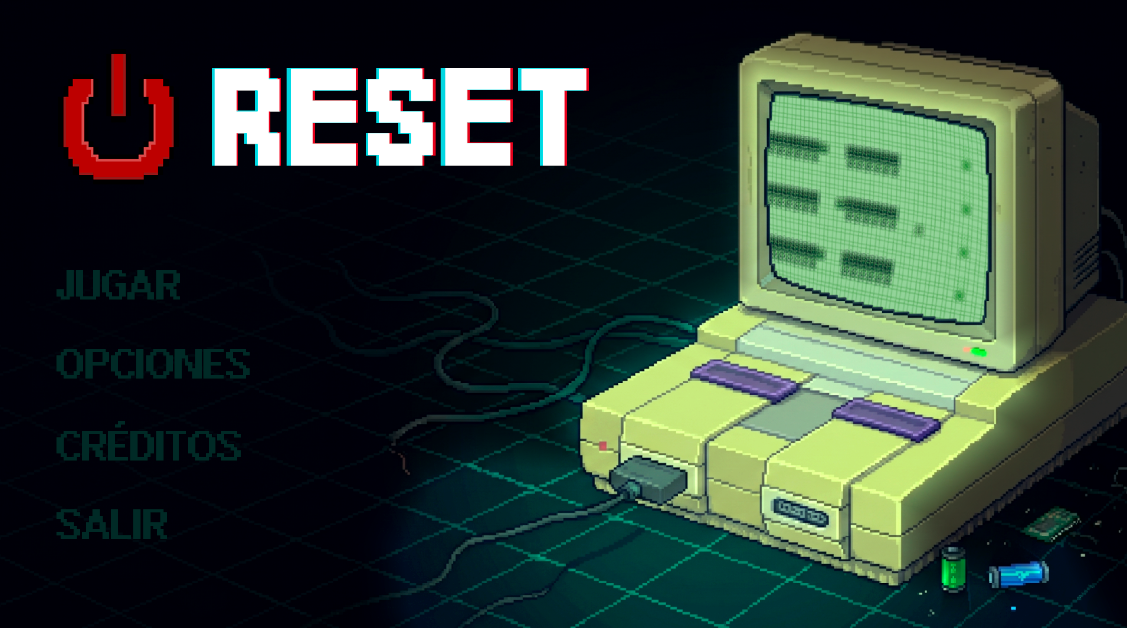
\includegraphics[width=0.75\textwidth]{pages/img/MainMenuReset.png}
    \caption{Menú principal de \textit{Reset}}
    \label{fig:ap:mainmenu}
\end{figure}

\begin{figure}[htbp]
    \centering
    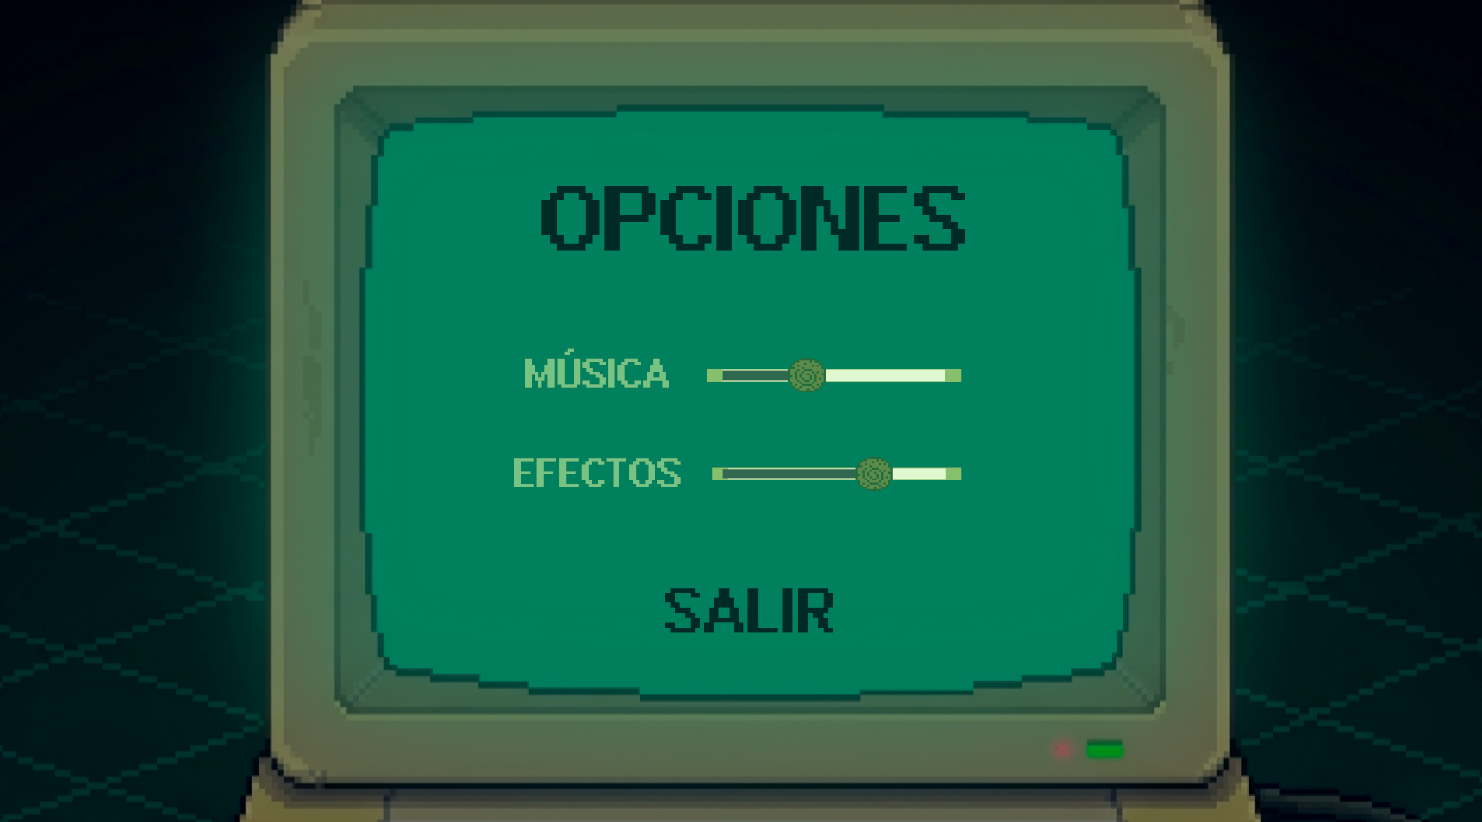
\includegraphics[width=0.75\textwidth]{pages/img/MainMenuOptions.png}
    \caption{Opciones del menú principal de \textit{Reset}}
    \label{fig:ap:mainmenuoptions}
\end{figure}

\clearpage
% =========================================================================
\section{El Nexo Central: El Hub y la Selección de Niveles}
El Hub actúa como nexo conector de la aventura. Desde esta zona, el jugador accede a las pantallas de selección de niveles y conversa con la consola para desbloquear el progreso de la historia:

\begin{figure}[htbp]
    \centering
    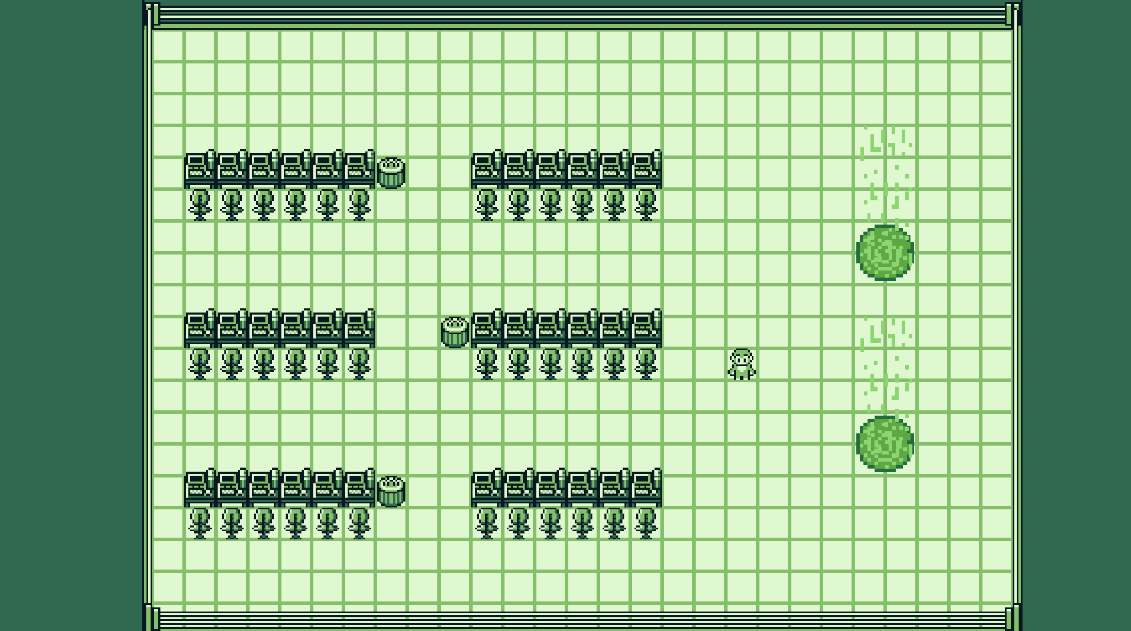
\includegraphics[width=0.75\textwidth]{pages/img/Hub}
    \caption{Diseño del escenario y punto de encuentro central (Hub).}
    \label{fig:ap:hub}
\end{figure}

\begin{figure}[htbp]
    \centering
    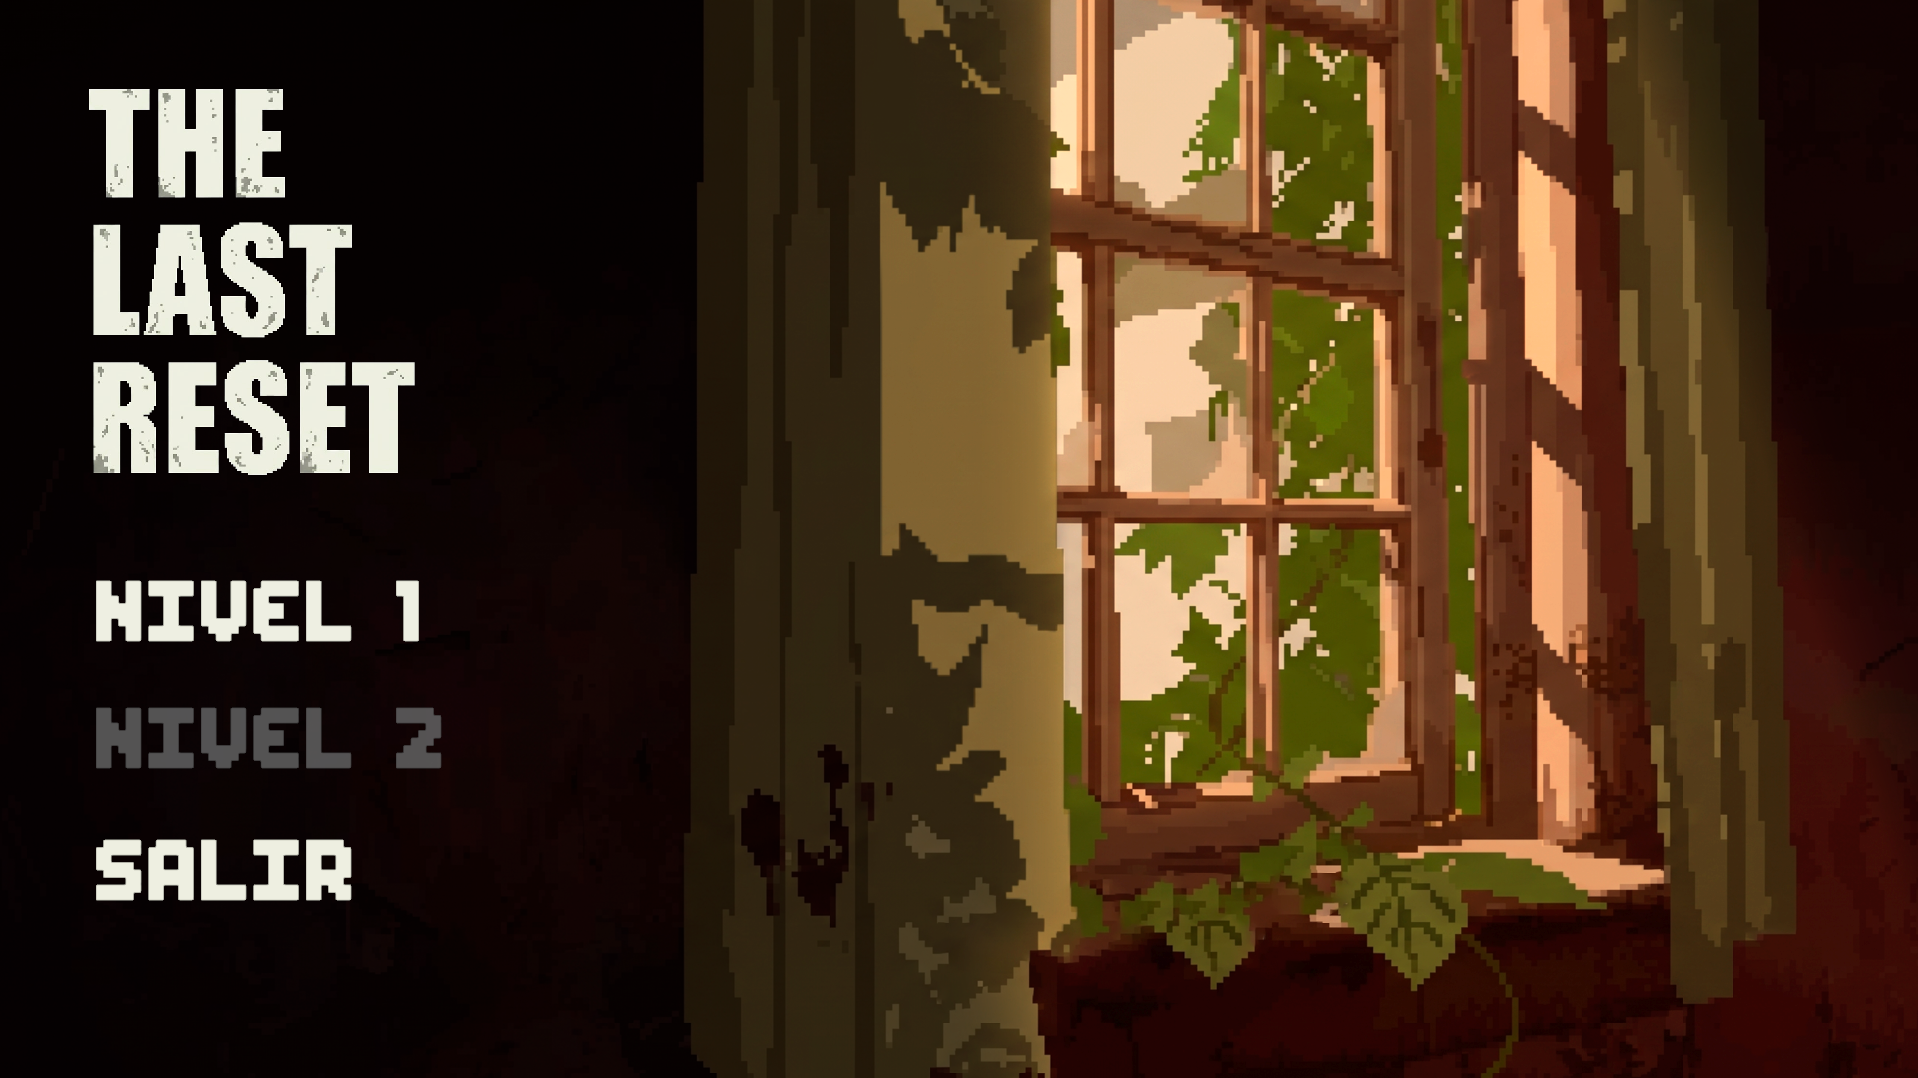
\includegraphics[width=0.75\textwidth]{pages/img/TheLastReset.png}
    \caption{Diseño del menú del mundo 1 \textit{The Last Reset.}}
    \label{fig:ap:tlrmenu}
\end{figure}

\begin{figure}[htbp]
    \centering
    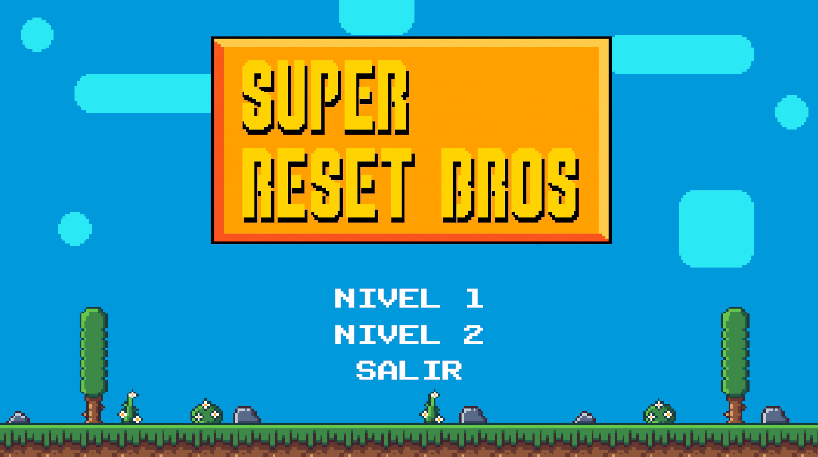
\includegraphics[width=0.75\textwidth]{pages/img/SuperResetBros.png}
    \caption{Diseño del menú del mundo 2 \textit{Super Reset Bros.}}
    \label{fig:ap:superresetbrosmenu}
\end{figure}

\begin{figure}[htbp]
    \centering
    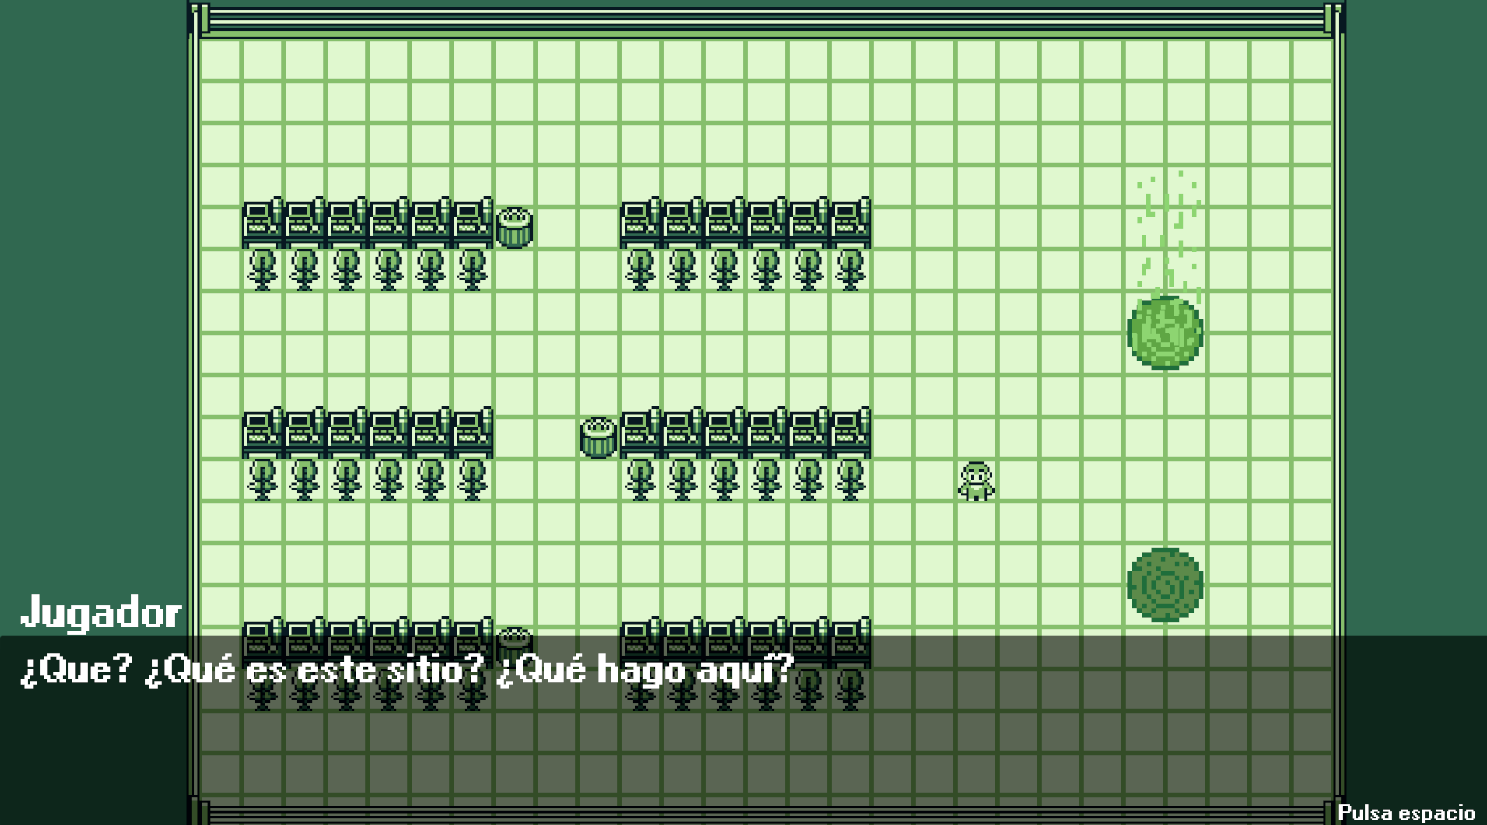
\includegraphics[width=0.75\textwidth]{pages/img/DialogueHub.png}
    \caption{Caja de diálogo interactiva con los NPC dentro del área del Hub.}
    \label{fig:ap:dialogo_hub}
\end{figure}

\begin{figure}[htbp]
    \centering
    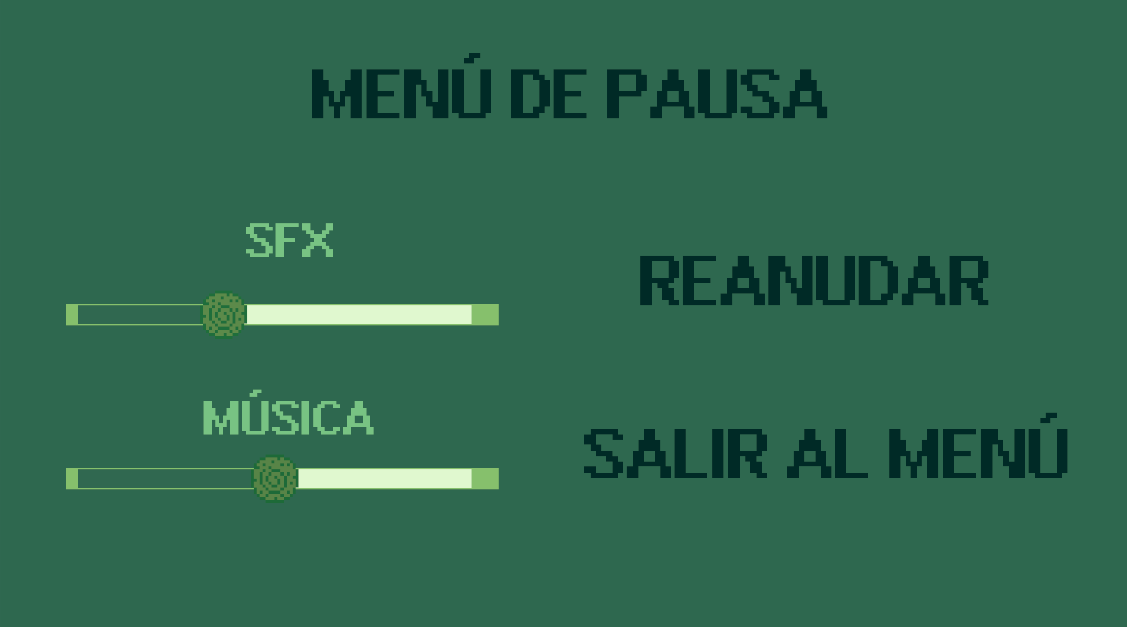
\includegraphics[width=0.75\textwidth]{pages/img/OptionsHub}
    \caption{Diseño de las opciones del Hub.}
    \label{fig:ap:optionshub}
\end{figure}

\clearpage
% =========================================================================
\section{Mundo 1: Entorno Cenital de Acción y Supervivencia}
Galería visual de los niveles del Mundo 1, mostrando la interfaz del inventario dinámico, los sistemas de diálogos de historia en el nivel y los escenarios de combate en perspectiva cenital:

\begin{figure}[htbp]
    \centering
    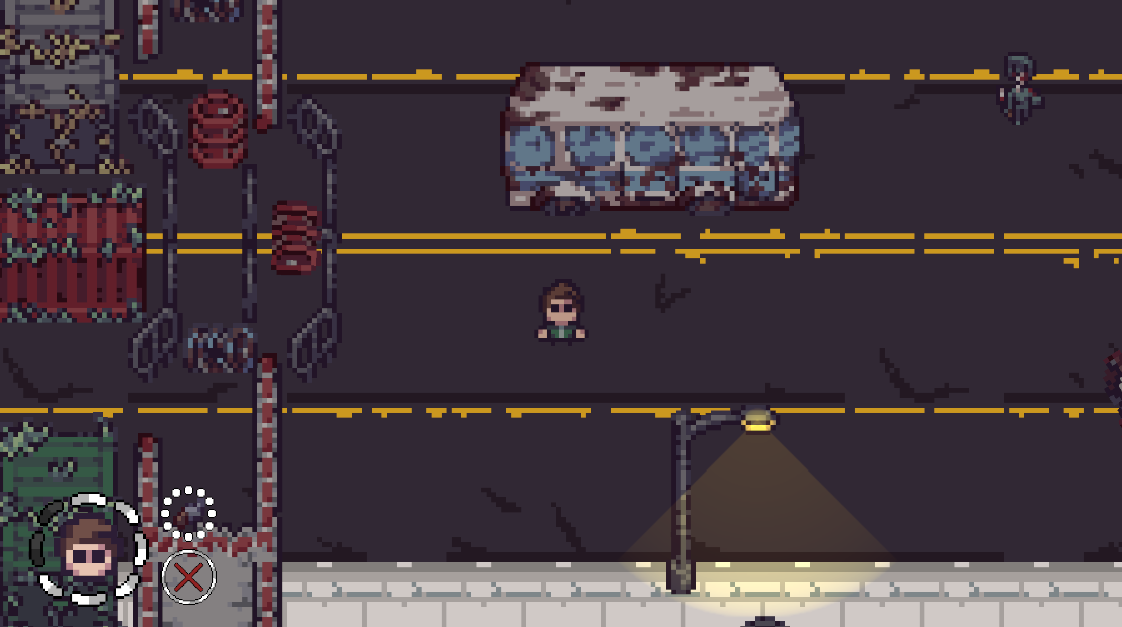
\includegraphics[width=0.75\textwidth]{pages/img/HUD1}
    \caption{Diseño del HUD del mundo 1.}
    \label{fig:ap:hud1}
\end{figure}

\begin{figure}[htbp]
    \centering
    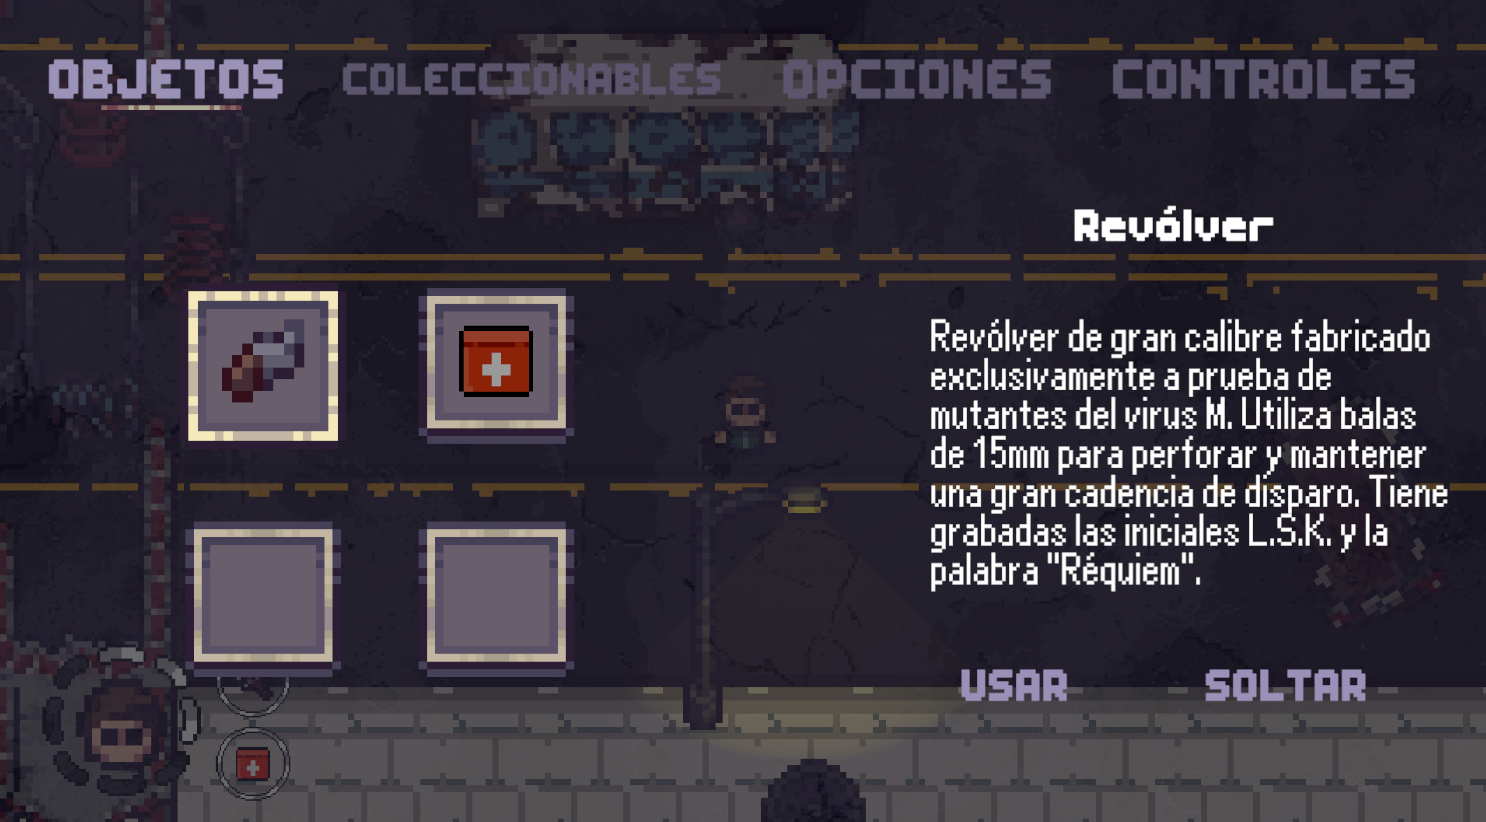
\includegraphics[width=0.75\textwidth]{pages/img/Inventario.png}
    \caption{Diseño del panel de Inventario del mundo 1.}
    \label{fig:ap:inventario}
\end{figure}

\begin{figure}[htbp]
    \centering
    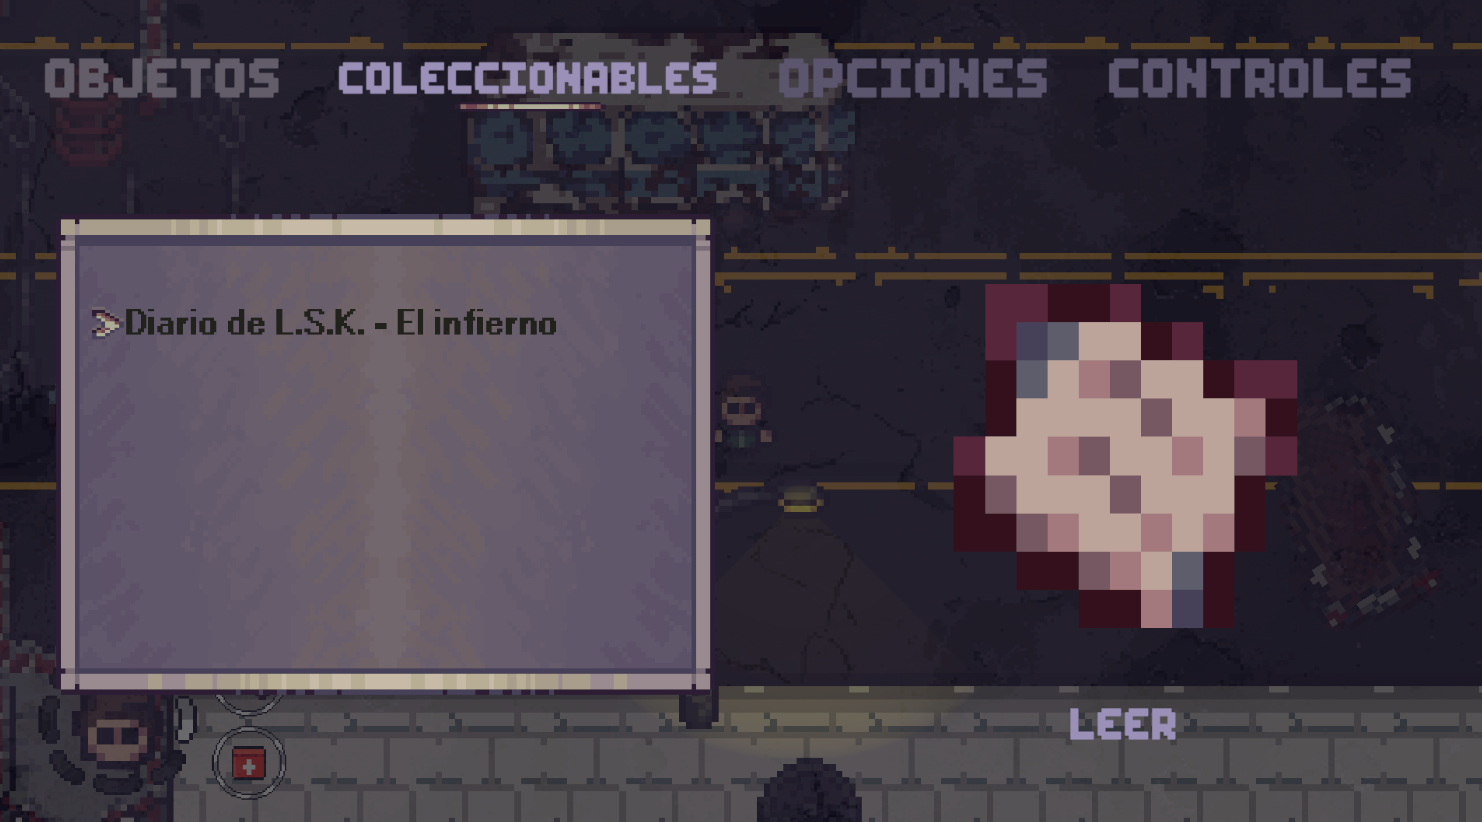
\includegraphics[width=0.75\textwidth]{pages/img/Coleccionables.png}
    \caption{Diseño del panel de Coleccionables del mundo 1.}
    \label{fig:ap:coleccionables}
\end{figure}

\begin{figure}[htbp]
    \centering
    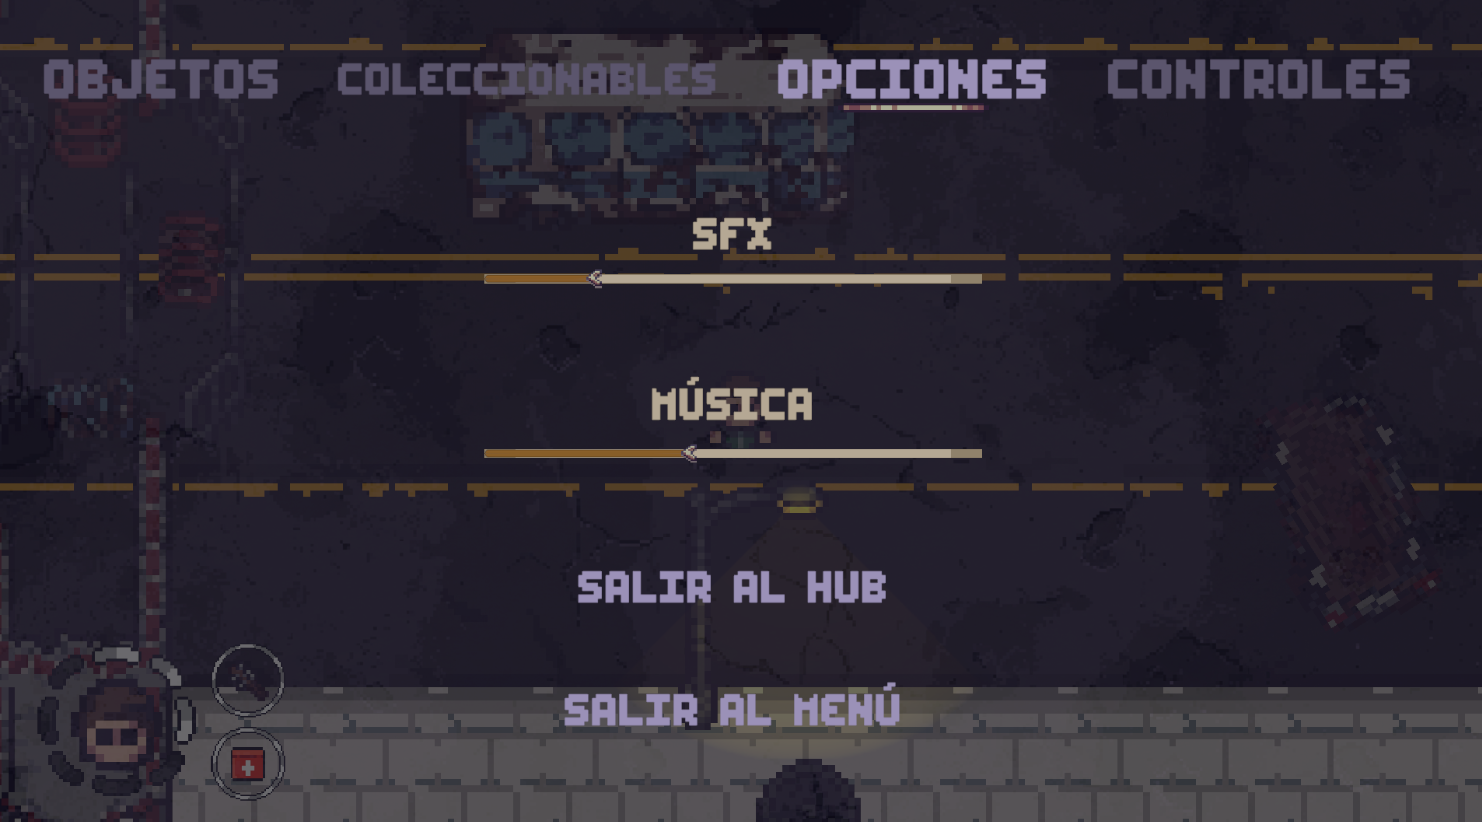
\includegraphics[width=0.75\textwidth]{pages/img/Opciones1.png}
    \caption{Diseño del panel de Opciones del mundo 1.}
    \label{fig:ap:opciones}
\end{figure}

\begin{figure}[htbp]
    \centering
    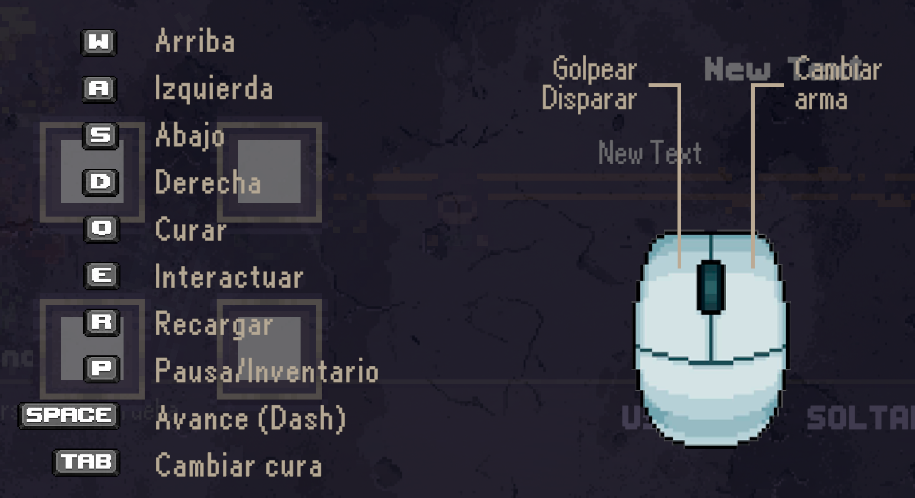
\includegraphics[width=0.75\textwidth]{pages/img/ControlesMundo1.png}
    \caption{Diseño del panel de Controles del mundo 1.}
    \label{fig:ap:controles}
\end{figure}

\begin{figure}[htbp]
    \centering
    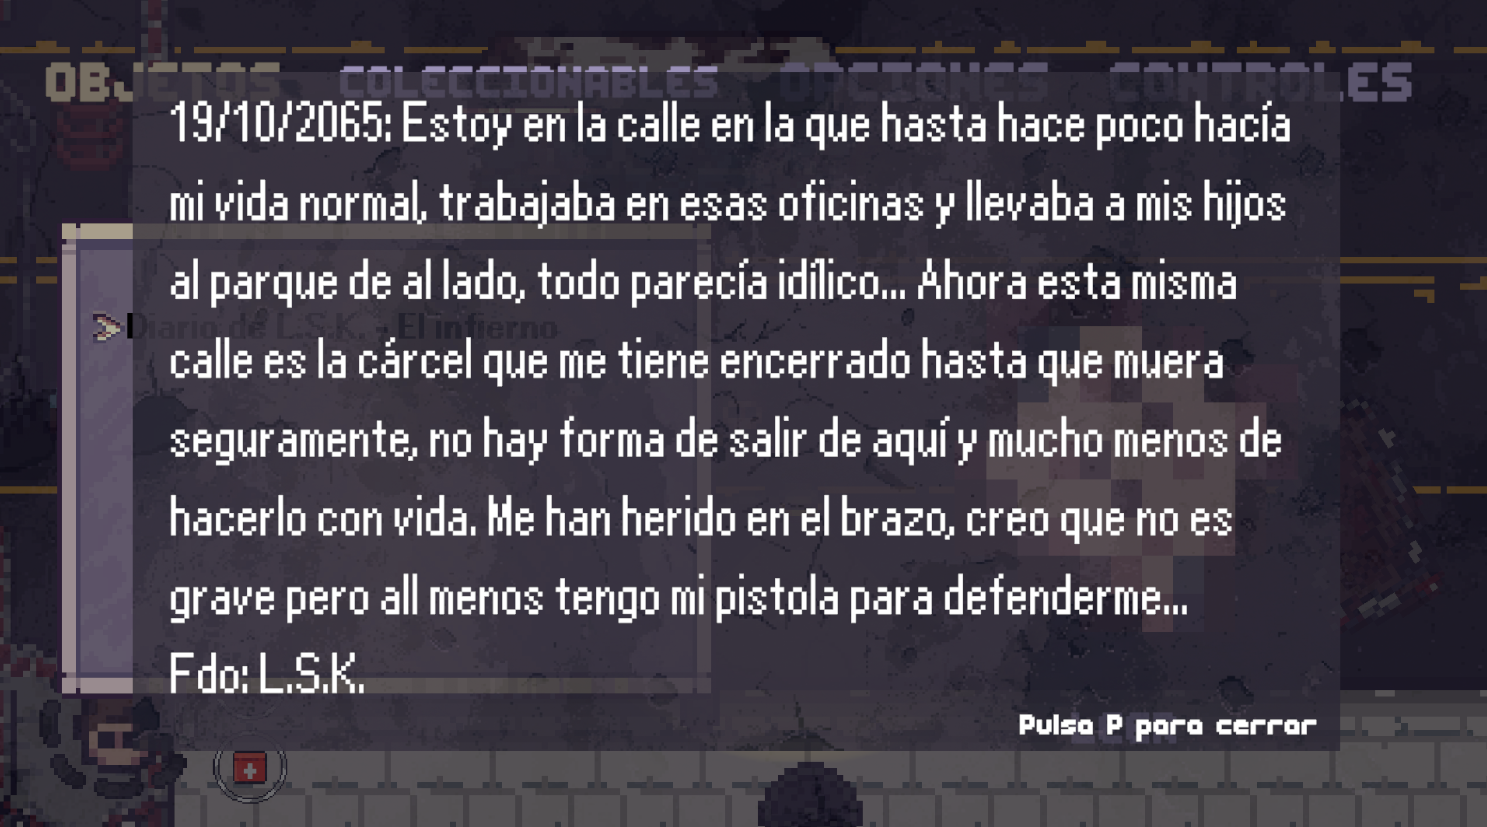
\includegraphics[width=0.75\textwidth]{pages/img/Notas.png}
    \caption{Diseño del panel de Notas del mundo 1.}
    \label{fig:ap:notes}
\end{figure}

\begin{figure}[htbp]
    \centering
    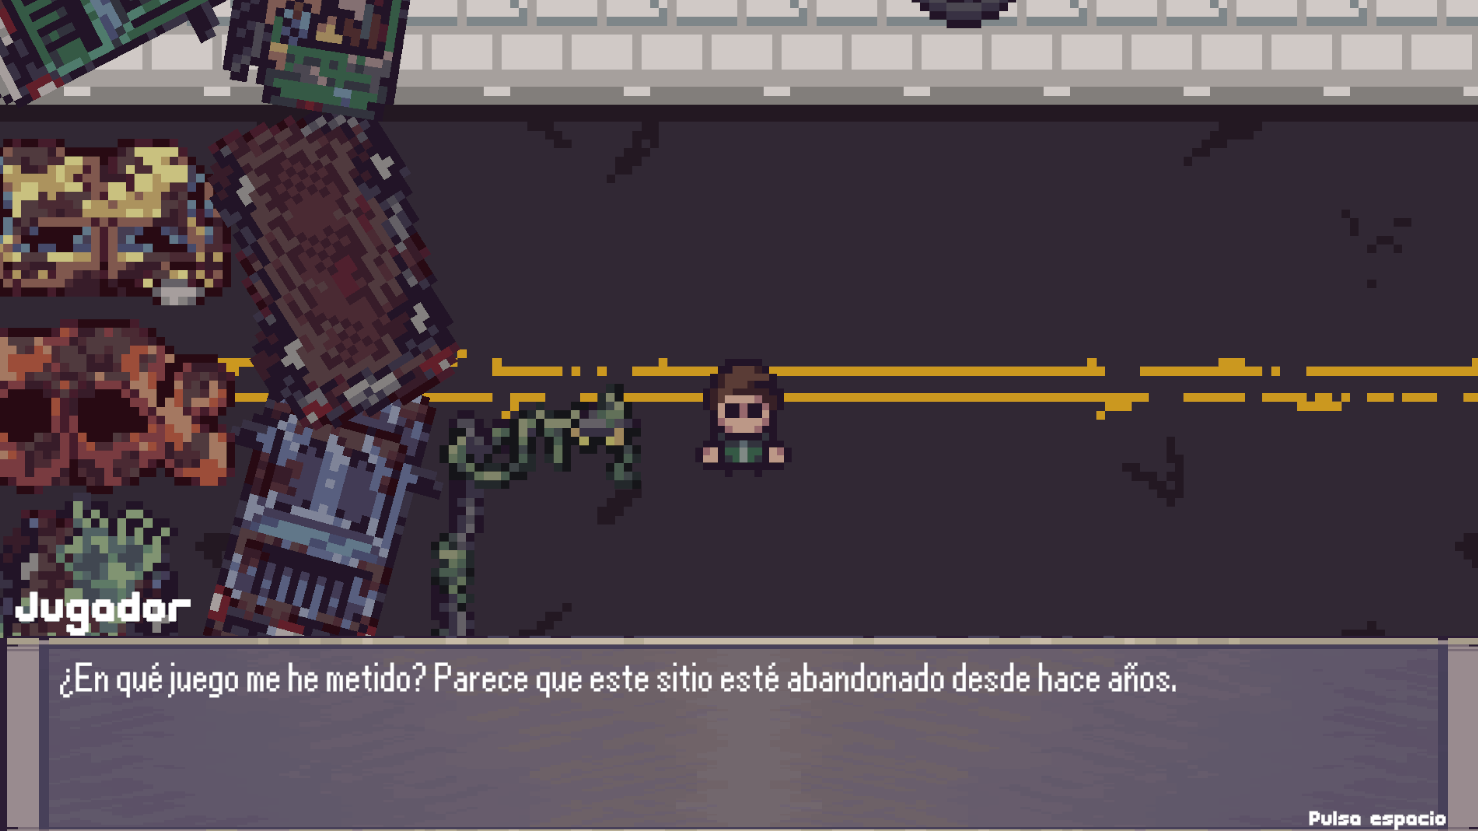
\includegraphics[width=0.75\textwidth]{pages/img/Dialogue1.png}
    \caption{Diseño del panel de Diálogo del mundo 1.}
    \label{fig:ap:dialogo1}
\end{figure}

\begin{figure}[htbp]
    \centering
    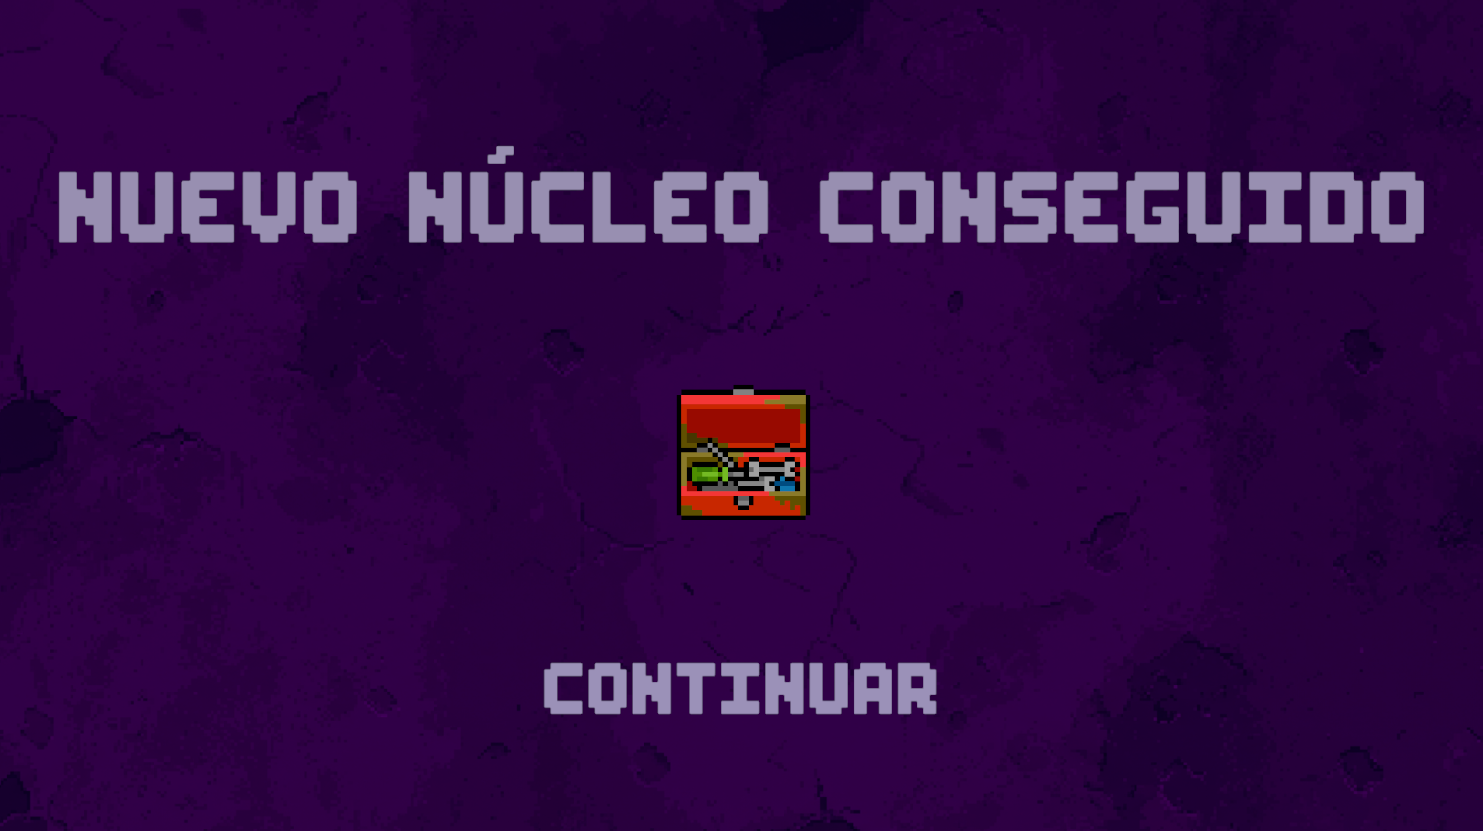
\includegraphics[width=0.75\textwidth]{pages/img/Victoria1.png}
    \caption{Diseño del panel de Victoria del mundo 1.}
    \label{fig:ap:victoria1}
\end{figure}

\begin{figure}[htbp]
    \centering
    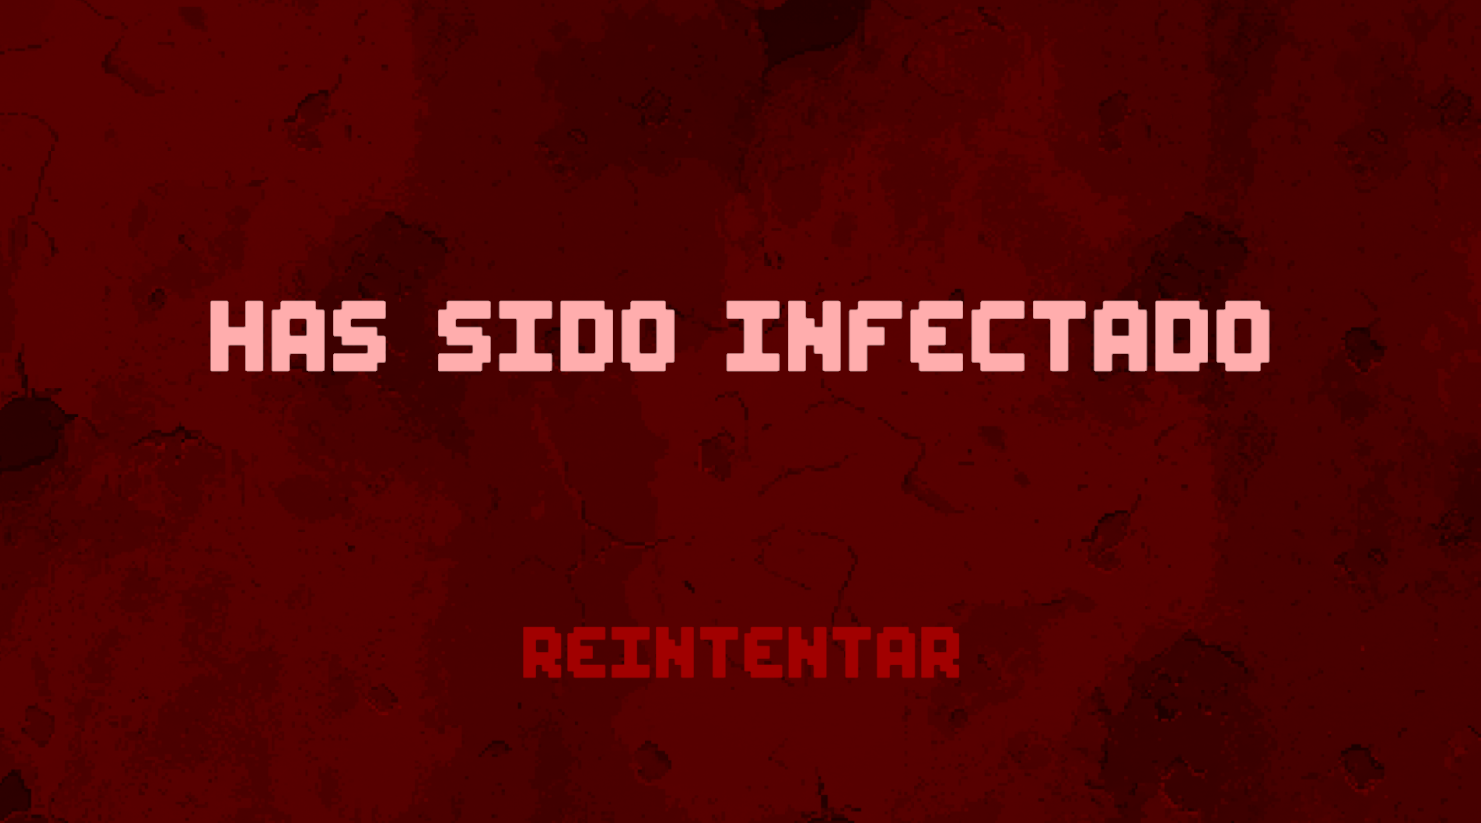
\includegraphics[width=0.75\textwidth]{pages/img/GameOver1.png}
    \caption{Diseño del panel de Derrota del mundo 1.}
    \label{fig:ap:gameover1}
\end{figure}

\begin{figure}[H]
    \centering
    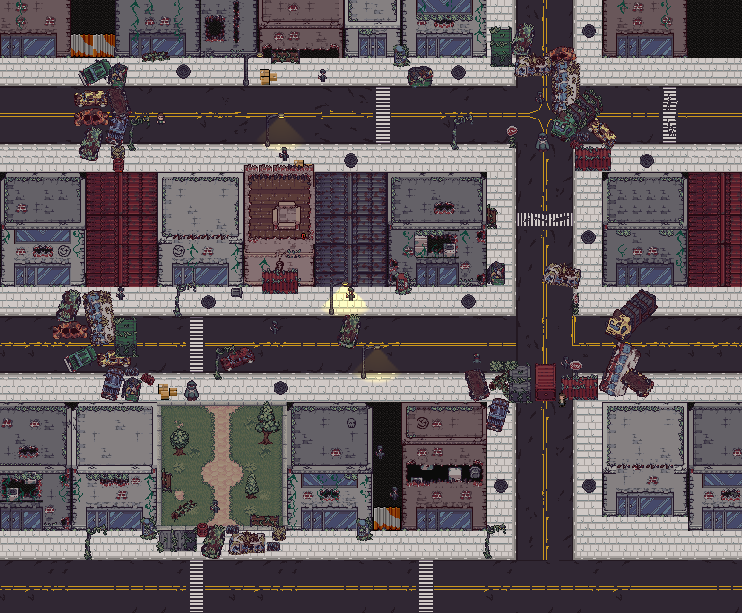
\includegraphics[width=0.75\textwidth]{pages/img/Nivel1.png}
    \caption{Diseño del nivel 1 del mundo 1.}
    \label{fig:ap:nivel11}
\end{figure}

\begin{figure}[H]
    \centering
    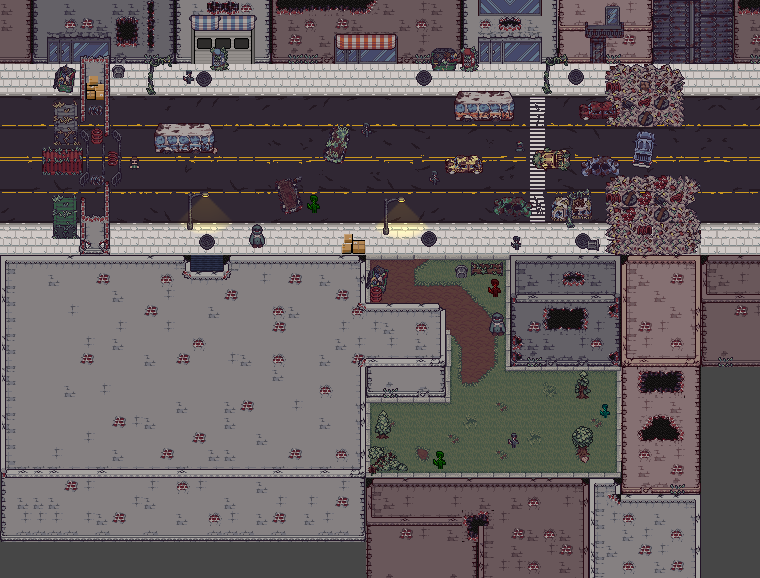
\includegraphics[width=0.75\textwidth]{pages/img/Nivel2.png}
    \caption{Diseño del nivel 2 del mundo 1.}
    \label{fig:ap:nivel121}
\end{figure}

\begin{figure}[H]
    \centering
    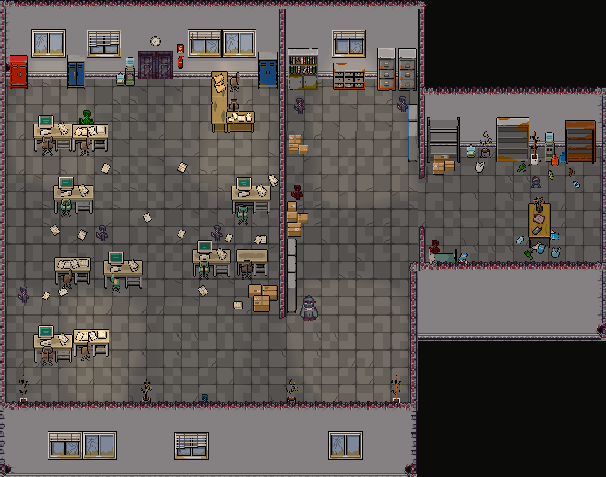
\includegraphics[width=0.75\textwidth]{pages/img/Nivel2.1.png}
    \caption{Diseño del nivel 2 del mundo 1.}
    \label{fig:ap:nivel122}
\end{figure}

\clearpage
% =========================================================================
\section{Mundo 2: Desafío de Plataformas Lateral}
Galería visual de los niveles del Mundo 2, mostrando el HUD con contadores de vidas, monedas y tiempo, los diálogos, interfaces y la extensión panorámica de los escenarios:

\begin{figure}[htbp]
    \centering
    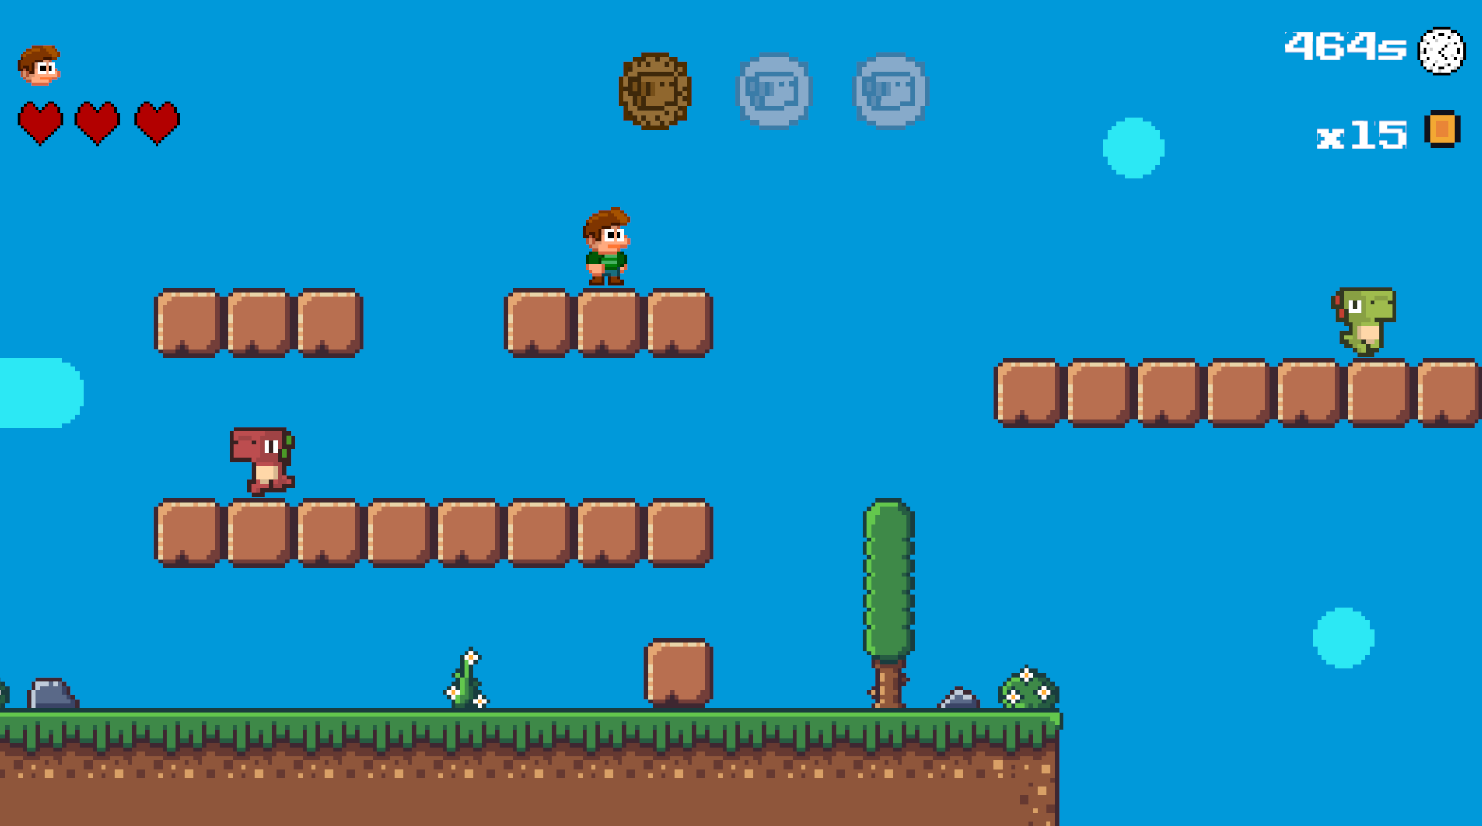
\includegraphics[width=0.75\textwidth]{pages/img/HUD2}
    \caption{Diseño del HUD del mundo 2.}
    \label{fig:ap:hud2}
\end{figure}

\begin{figure}[htbp]
    \centering
    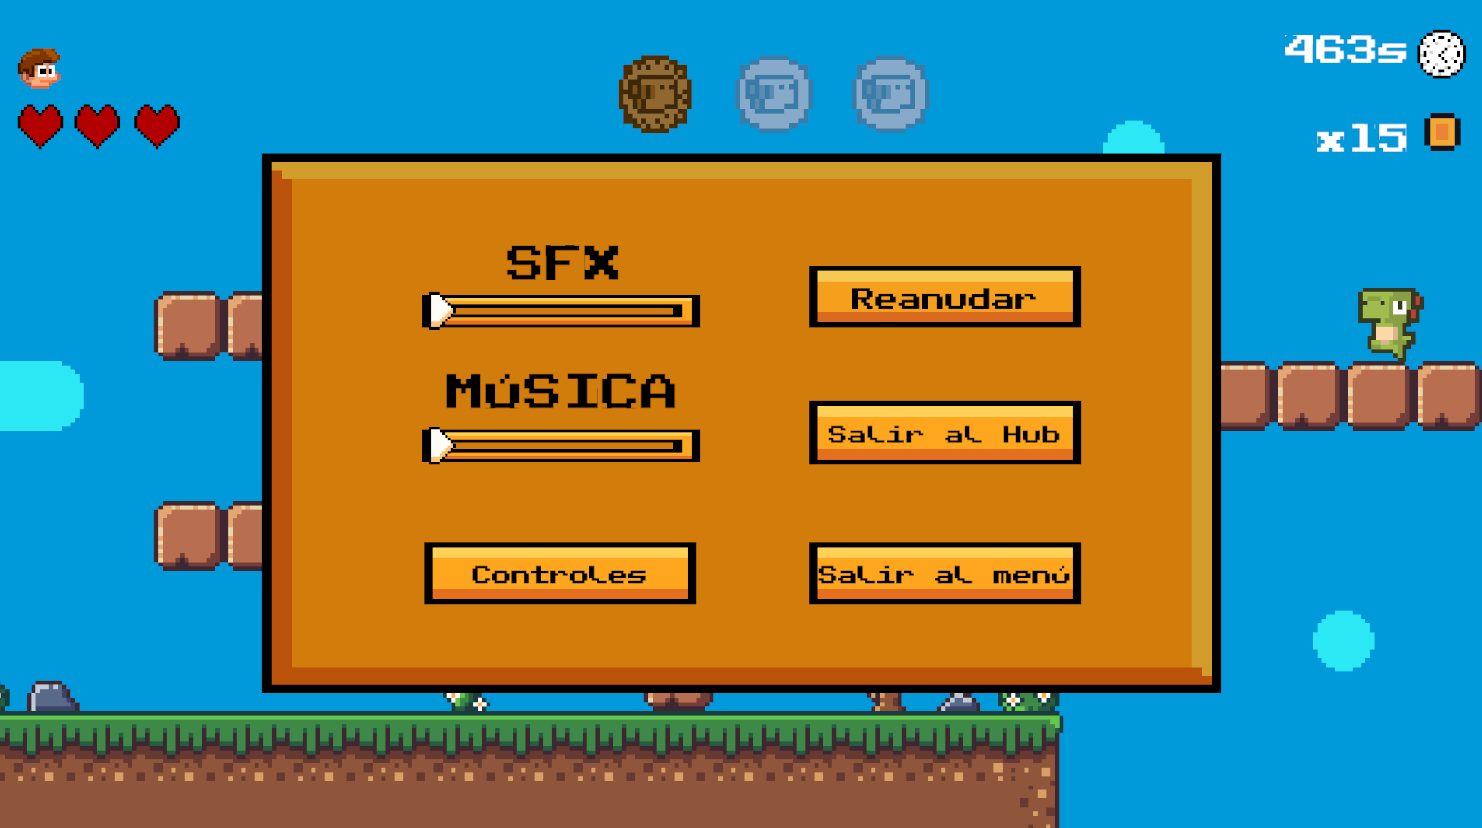
\includegraphics[width=0.75\textwidth]{pages/img/Opciones2.png}
    \caption{Diseño del panel de Opciones del mundo 2.}
    \label{fig:ap:opciones2}
\end{figure}

\begin{figure}[htbp]
    \centering
    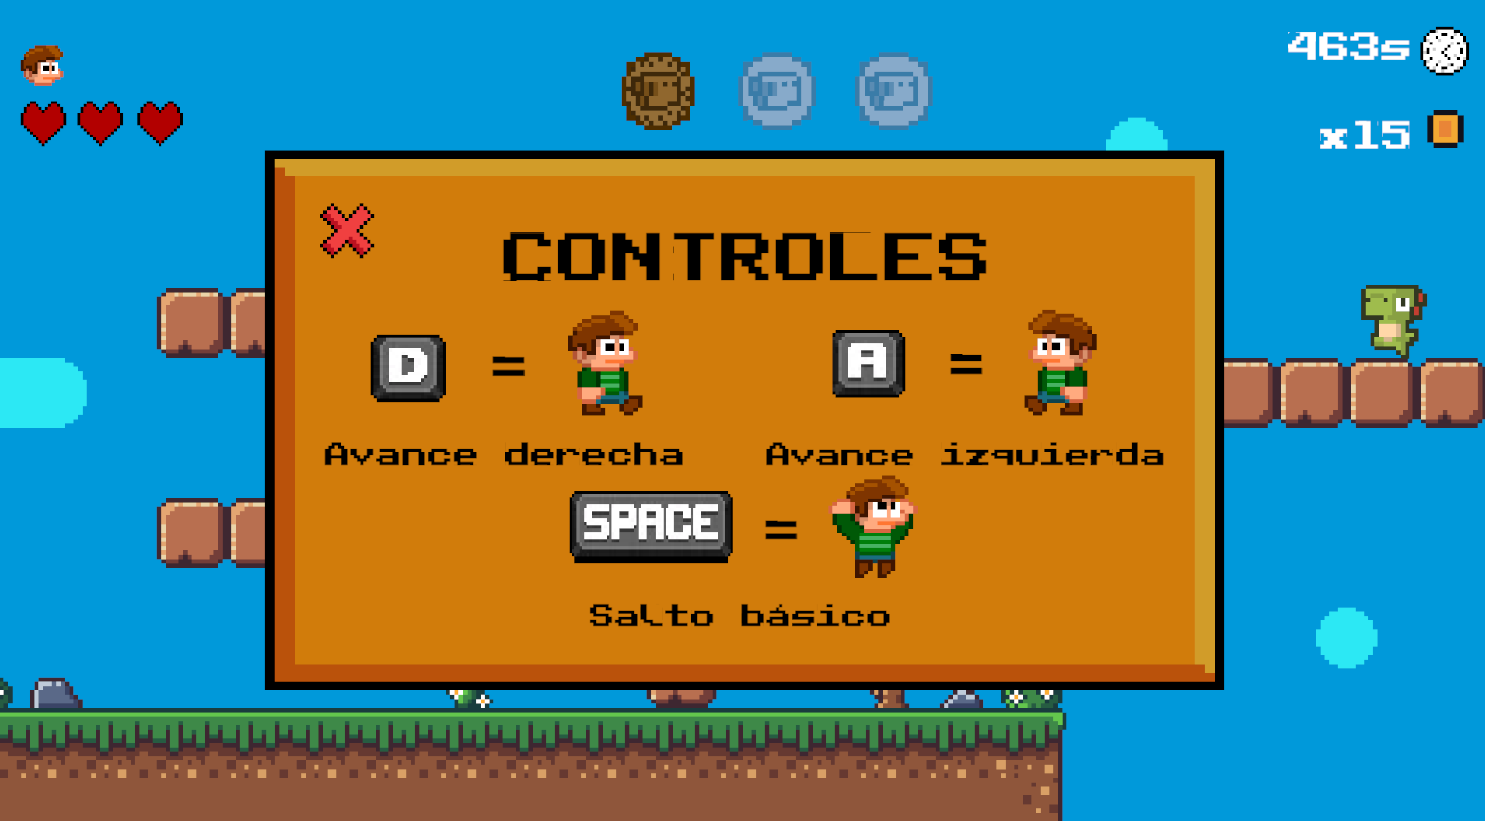
\includegraphics[width=0.75\textwidth]{pages/img/Controles2.png}
    \caption{Diseño del panel de Controles del nivel 1 mundo 2.}
    \label{fig:ap:controles2.1}
\end{figure}

\begin{figure}[htbp]
    \centering
    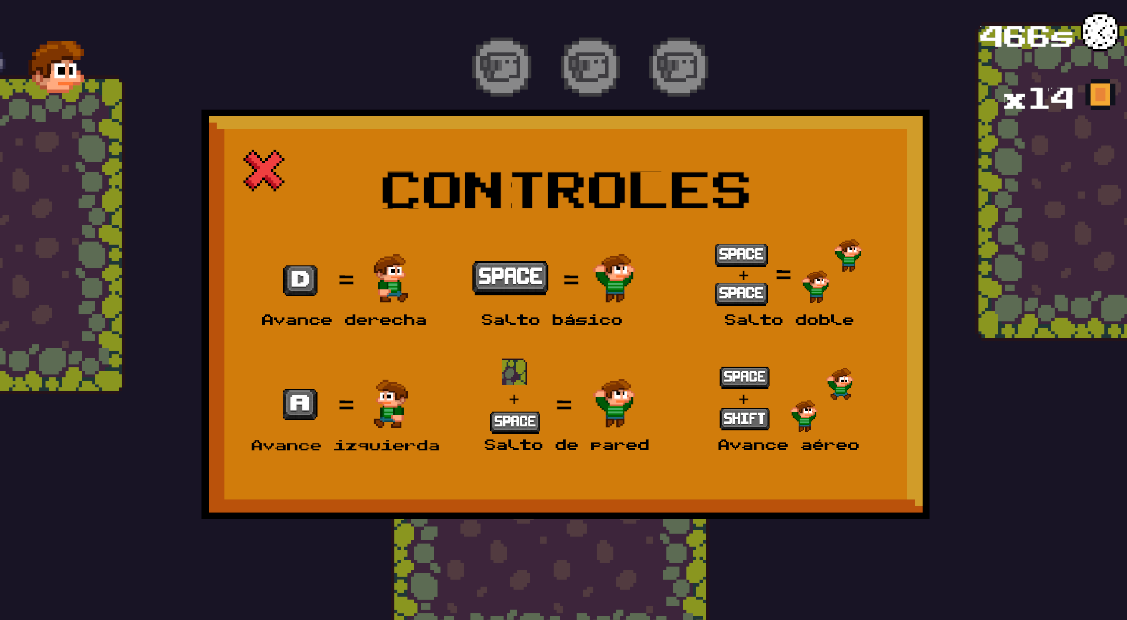
\includegraphics[width=0.75\textwidth]{pages/img/Controles3.png}
    \caption{Diseño del panel de Controles del nivel 2 mundo 2.}
    \label{fig:ap:controles2.2}
\end{figure}

\begin{figure}[htbp]
    \centering
    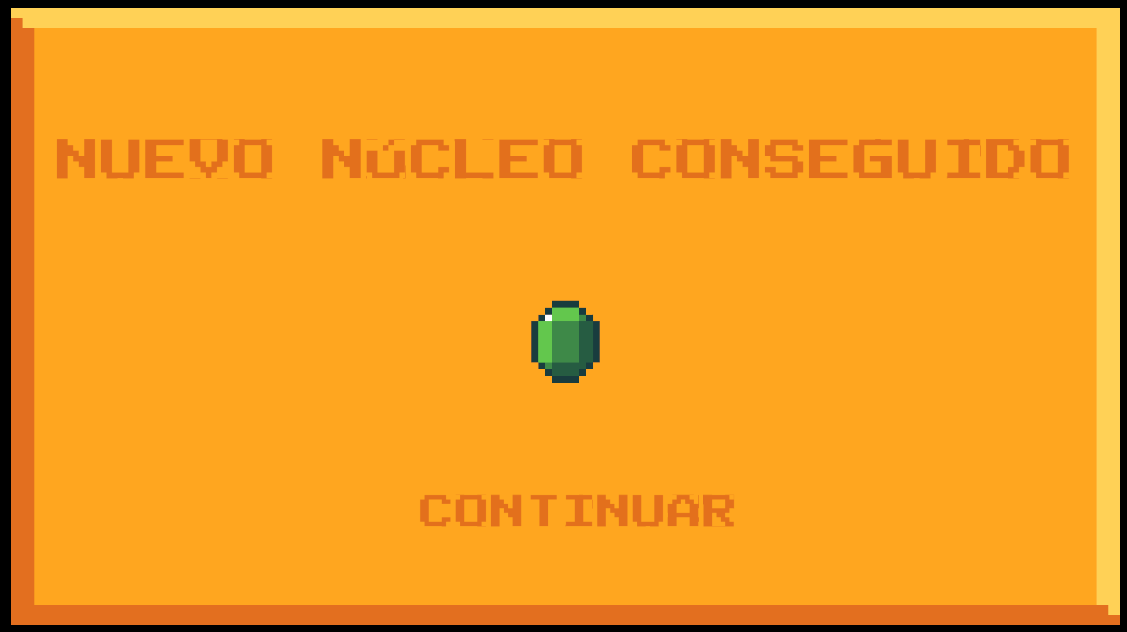
\includegraphics[width=0.75\textwidth]{pages/img/Victoria2.png}
    \caption{Diseño del panel de Victoria del mundo 2.}
    \label{fig:ap:victoria2}
\end{figure}

\begin{figure}[htbp]
    \centering
    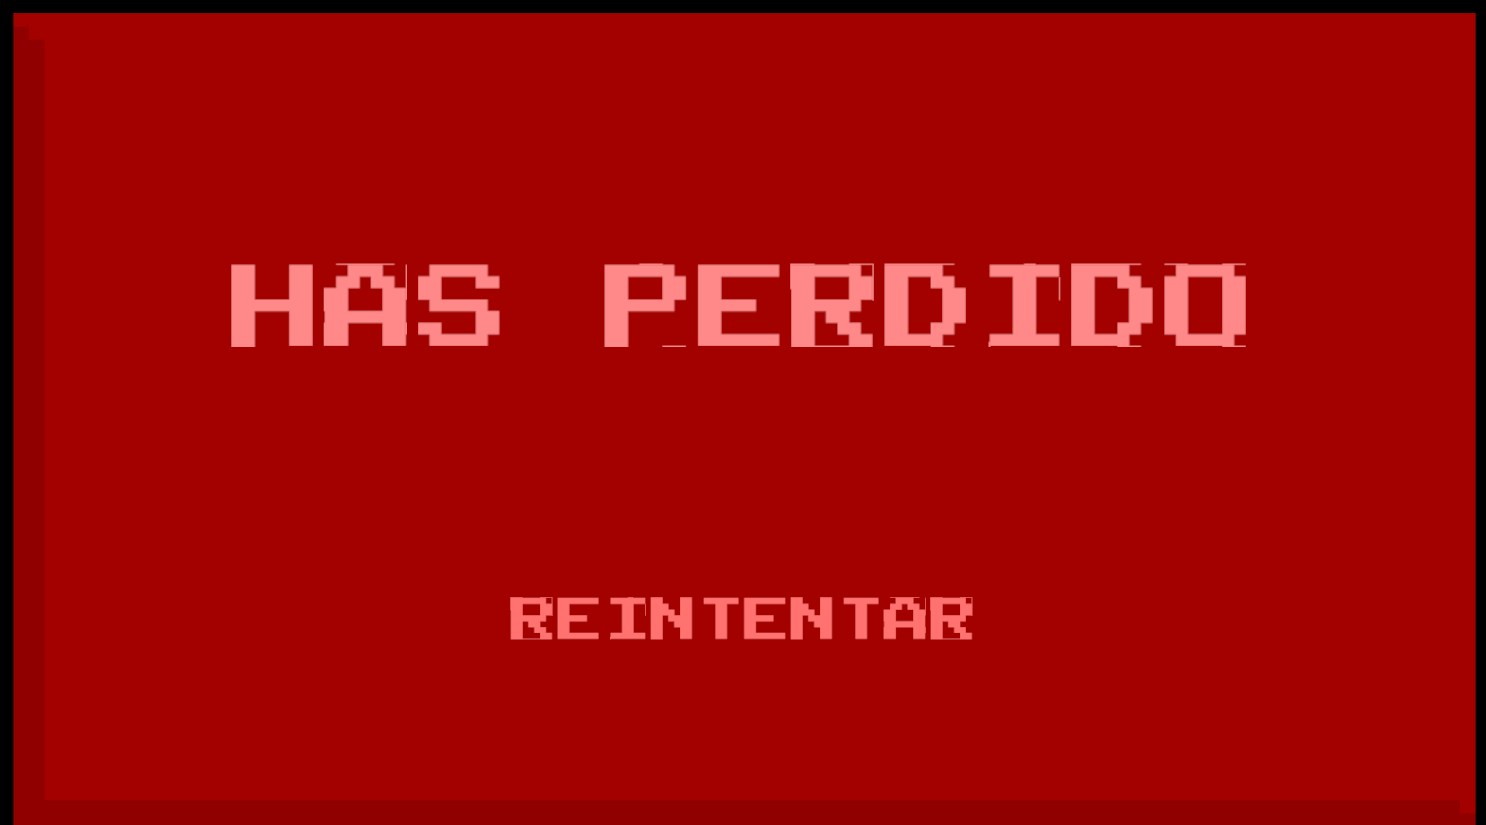
\includegraphics[width=0.75\textwidth]{pages/img/GameOver2.png}
    \caption{Diseño del panel de Derrota del mundo 2.}
    \label{fig:ap:derrota2}
\end{figure}

\begin{figure}[htbp]
    \centering
    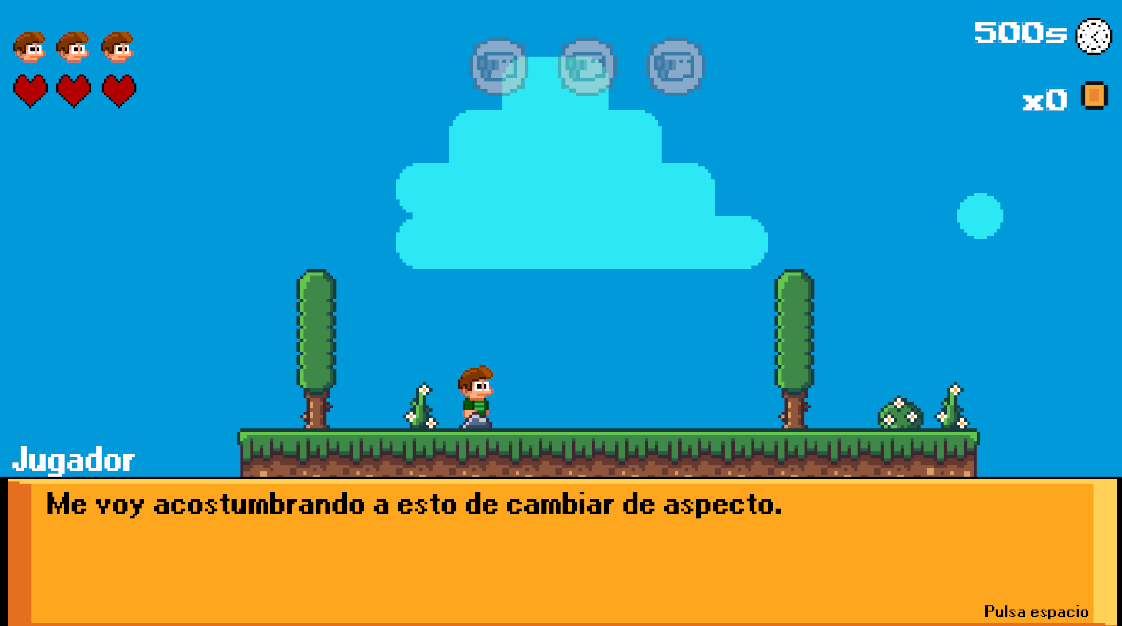
\includegraphics[width=0.75\textwidth]{pages/img/Dialogue2.png}
    \caption{Diseño del panel de Diálogo del mundo 2.}
    \label{fig:ap:dialogo2}
\end{figure}

\begin{figure}[htbp]
    \centering
    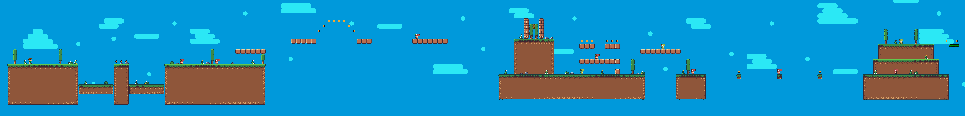
\includegraphics[width=0.9\textwidth]{pages/img/Mundo2.1.1.png}
    \caption{Diseño del nivel 1 del mundo 2.}
    \label{fig:ap:mundo211}
\end{figure}

\begin{figure}[htbp]
    \centering
    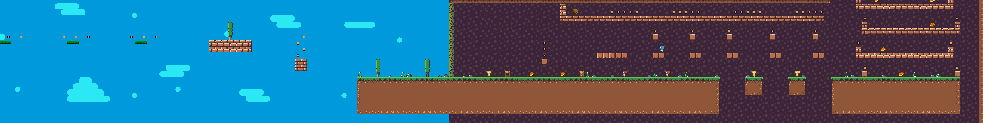
\includegraphics[width=0.9\textwidth]{pages/img/Mundo2.1.2.png}
    \caption{Diseño del nivel 1 del mundo 2.}
    \label{fig:ap:mundo212}
\end{figure}

\begin{figure}[htbp]
    \centering
    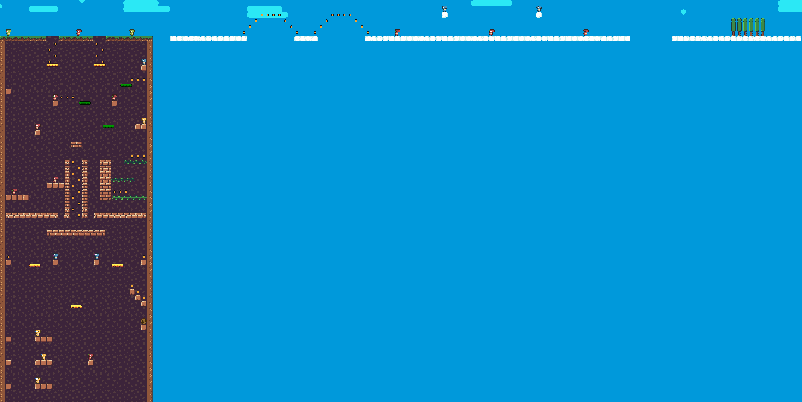
\includegraphics[width=0.75\textwidth]{pages/img/Mundo2.1.3.png}
    \caption{Diseño del nivel 1 del mundo 2.}
    \label{fig:ap:mundo213}
\end{figure}

\begin{figure}[htbp]
    \centering
    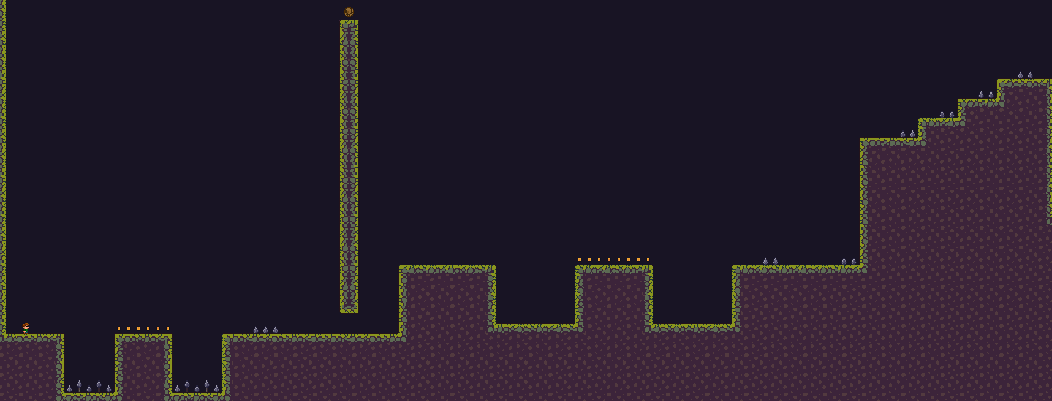
\includegraphics[width=0.75\textwidth]{pages/img/Mundo2.2.1.png}
    \caption{Diseño del nivel 2 del mundo 2.}
    \label{fig:ap:mundo221}
\end{figure}

\begin{figure}[htbp]
    \centering
    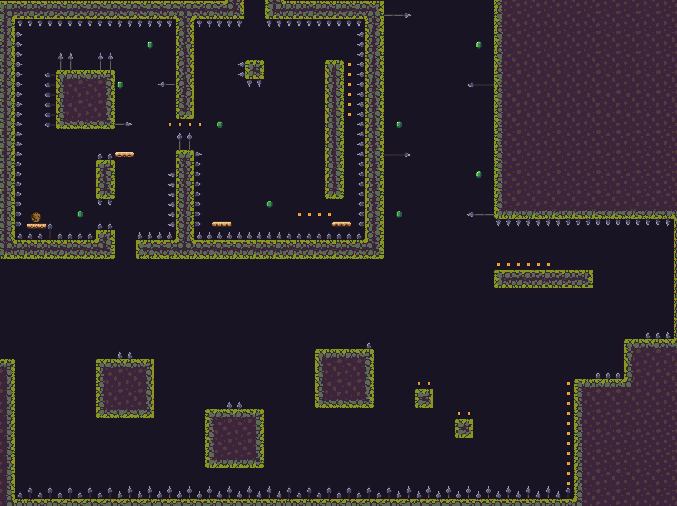
\includegraphics[width=0.75\textwidth]{pages/img/Mundo2.2.2.png}
    \caption{Diseño del nivel 2 del mundo 2.}
    \label{fig:ap:mundo222}
\end{figure}

\begin{figure}[htbp]
    \centering
    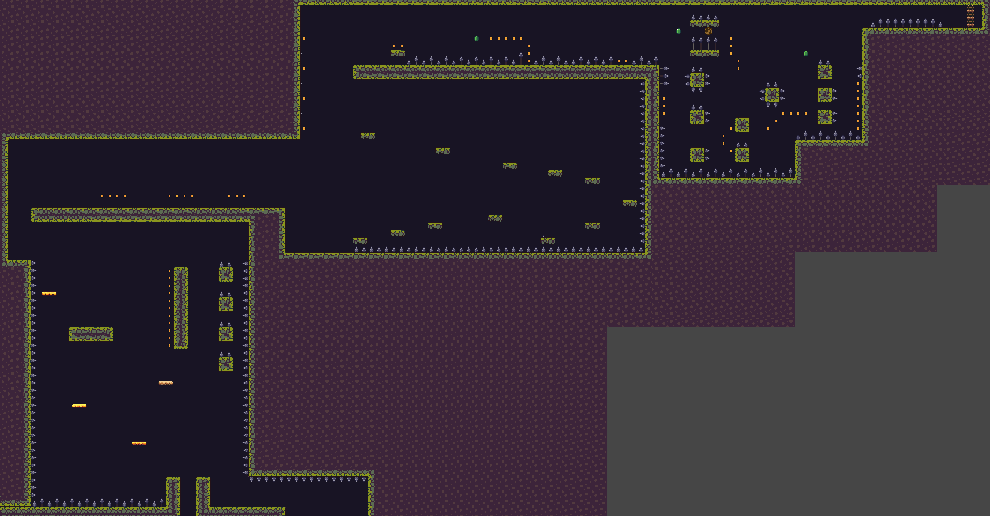
\includegraphics[width=0.75\textwidth]{pages/img/Mundo2.2.3.png}
    \caption{Diseño del nivel 2 del mundo 2.}
    \label{fig:ap:mundo223}
\end{figure}